\scanpage{106}
\mspage{105}%
i.e. that the filtration of the said functor a\unsure{\rlap{m}d|d}\rlap{d}mits a\deleted{e} splitting compatible with tensor products. But the choice of such a splitting is equivalent to that of a point \deleted{under} on a certain right torsor $Q=Q'$ under the group \inserted{
\begin{tikzpicture}[baseline=-.2ex,x=1em,y=1em]
\node[anchor=base west] at (0,.4) {scheme};
\draw (-.15,.6) .. controls (-.3,.1) and (.2,0) .. (1,0) -- (2.5,.05) .. controls (3.1,.05) and (3.5,-.1) .. (3.6,-.6) .. controls (3.8,.05) and (4.1,.05) .. (4.7,.1) -- (5.8,.3) .. controls (6.2,.4) and (6.2,.5) .. (6.1,.65);
\end{tikzpicture}} \inserted{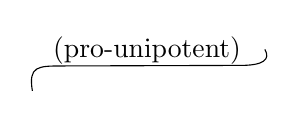
\begin{tikzpicture}[baseline=-.2ex,x=1em,y=1em]
\node[anchor=base west] at (0,.4) {(pro-unipotent)};
\draw (-.4,-.8) .. controls (-.55,.1) and (-.2,.1) .. (.7,.1) -- (7,.12) .. controls (8,.1) and (8.2,.35) .. (8,.7);
\end{tikzpicture}} $H$ of automorphisms of $F$ preserving the filtration and inducing the identity on the associated graded; it is not at all canonical !

3) Let us call a \uline{pre-Hodge str\rlap{c}u\rlap{u}cture} on a vector space \inserted{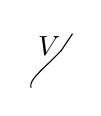
\begin{tikzpicture}[baseline=-.2ex,x=1em,y=1em]
\node[anchor=base west] at (0,.5) {$V$};
\draw (.1,-.65) .. controls (0,-.35) and (.6,.05) .. (1.2,.7) -- (1.6,1.3);
\end{tikzpicture}} of finite dimension over $\underline{Q}$, the datum of a bigrading on $V\otimes_{\underline{Q}}\underline{C}=V_{\underline{C}}$, $V_{\underline{C}}=\handwritten{\coprod_{p,q}}V^{p,q}$, such that a) the corresponding total grading is ``defined over $\underline{Q}$'' \uline{i.e.} $\handwritten{\coprod}_{p+q=n}V^{p,q}$ comes from a subspace $V_{\underline{Q}}^n$ of $V$, and b) one has $\overset{\handwritten{\rule{.65em}{.35pt}}}{V}^{p,q}=V^{q,p}$, where $x\handwritten{\mapsto}\overset{\handwritten{\rule{.55em}{.35pt}}}{x}$ denotes complex conjugation. \unsure{(}NB Generalization to more general fields left to Saavedra). The vector spaces $V$ equipped with a pre-Hodge structure form a tensor category over $\underline{Q}$ in an obvious sense, equipped with a canonical fibre functor, the ``forgetful'' functor\inserted{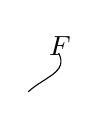
\begin{tikzpicture}[baseline=-.2ex,x=1em,y=1em]
\node[anchor=base west] at (0,.4) {$F$};
\draw (.7,.5) .. controls (1.05,-.2) and (.2,-.35) .. (-.4,-.9);
\end{tikzpicture}}. One thus finds a \unsure{$\mathbb{G}$|G}alois group $G$, and \deleted{every} more generally every \inserted{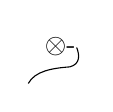
\begin{tikzpicture}[baseline=-.2ex,x=1em,y=1em]
\node[anchor=base west] at (0,.4) {$\otimes$-};
\draw (-.25,-.7) .. controls (0,-.25) and (.6,-.15) .. (1.25,-.1) .. controls (1.65,0) and (1.6,.35) .. (1.5,.6);
\end{tikzpicture}}subcategory $\underline{C}$ of the preceding category defines for us a Galois group $G$. The bigrading on the \deleted{forgetful} functor $F_{\underline{C}}(V)=V\otimes_{\underline{Q}}\underline{C}$ corresponds, by virtue of 1) (where it is however appropriate to allow oneself an extension of the base field on the fibre functor considered ....) of a homomorphism ${\underline{G}_m}_{\underline{C}}^2\handwritten{\longrightarrow}G_{\underline{C}}$, i.e. of two homomorphisms \inserted{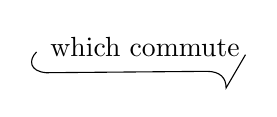
\begin{tikzpicture}[baseline=-.2ex,x=1em,y=1em]
\node[anchor=base west] at (0,.5) {which commute};
\draw (-.15,.65) .. controls (-.45,.35) and (-.4,-.05) .. (.2,-.1) -- (6,-.05) .. controls (6.5,-.05) and (6.7,-.3) .. (6.7,-.65) -- (7.4,.55);
\end{tikzpicture}}
\[
i_1,i_2:{\underline{G}_m}_{\underline{C}}\handwritten{\longrightarrow}G_{\underline{C}}.
\]
The two conditions a) and b) imposed on the structures considered are interpreted respectively by the facts that the homomorphism
\[
i_{\underline{C}}=i_1i_2\unsure{\doteqdot|=}\handwritten{\lambda\mapsto}i_1(\handwritten{\lambda})i_2(\handwritten{\lambda})
\]
is ``defined over $\underline{Q}$'' i.e. comes from a homomorphism
\[
i:\underline{G}_m\handwritten{\longrightarrow}G,
\]
\margin{\tikz[baseline=0pt,x=1em,y=1em]{\draw (0,0) .. controls (.1,.05) and (.17,.15) .. (.22,.3);}}(necessarily central, for the homogeneous components $V_{\underline{Q}}^n$ of a pre-Hodge structure are \deleted{necessarily}\inserted{obviously} equipped with a \inserted{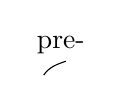
\begin{tikzpicture}[baseline=-.2ex,x=1em,y=1em]
\node[anchor=base west] at (0,.4) {pre-};
\draw (.6,-.55) .. controls (.8,-.25) and (1.1,-.15) .. (1.4,-.05);
\end{tikzpicture}}Hodge structure in such a way that $V$ is the direct sum of $V_{\underline{Q}}^n$ as a pre-structure
